\documentclass[draft,pdflatex,compress,svgnames,mathserif,serif]{beamer}
% BEAMERTHEME?
% \usetheme[dark, framenumber, totalframenumber]{UniversiteitAntwerpen}
\usetheme[orchid]{Singapore}
\setbeamertemplate{footline}{
    \leavevmode%
    \hbox{%
        \begin{beamercolorbox}[wd=.4\paperwidth,ht=2.25ex,dp=1ex]{author in head/foot}%
            \usebeamerfont{author}\hspace{1em}\insertshortauthor
        \end{beamercolorbox}%
        \begin{beamercolorbox}[wd=.6\paperwidth,ht=2.25ex,dp=1ex,right]{title in head/foot}%
            %\usebeamerfont{title in head/foot}\insertshorttitle\hspace*{3em}
            \usebeamerfont{frame number}\insertframenumber{} / \inserttotalframenumber\hspace*{1em}
        \end{beamercolorbox}}%
    \vskip0pt%
}

%[frame number]
\setbeamertemplate{navigation symbols}{}

% \AtBeginSection{\frame{\sectionpage}}

%%% Local Variables: 
%%% mode: latex
%%% TeX-master: "../main"
%%% End: 

% % without this multicol will not work in beamer
\usepackage{etex}

%%% Local Variables: 
%%% mode: latex
%%% TeX-master: "../../main"
%%% End: 

\usepackage[utf8]{inputenc}

%%% Local Variables: 
%%% mode: latex
%%% TeX-master: "../../main"
%%% End: 

\usepackage[T1]{fontenc}

%%% Local Variables: 
%%% mode: plain-tex
%%% TeX-master: "../../main"
%%% End: 

\usepackage{tikz}
\usetikzlibrary{arrows}
\usetikzlibrary{snakes}
\usetikzlibrary{backgrounds}
\usetikzlibrary{patterns}
\usetikzlibrary{matrix}
\usetikzlibrary{shapes}
\usetikzlibrary{fit}
\usetikzlibrary{calc}
\usetikzlibrary{shadows}
\usetikzlibrary{plotmarks}
\usetikzlibrary{positioning}
\usetikzlibrary{fadings}
\usetikzlibrary{shapes.arrows}

% transparent
\tikzstyle{transparent_node} = [draw, circle, opacity=0.3, fill, minimum width=17pt]
\tikzstyle{assignment_arrow} = [line width=1.2pt, ->, >=stealth, opacity=0.85]


% layers
\pgfdeclarelayer{lower}
\pgfdeclarelayer{upper}
\pgfdeclarelayer{bglower}
\pgfdeclarelayer{bgupper}
\pgfdeclarelayer{transition}
\pgfsetlayers{background,bglower,lower,transition,bgupper,upper,main}


% GMM
\tikzstyle{main}=[circle, minimum size = 10mm, thick, draw =black!80, node distance = 16mm]
\tikzstyle{param}=[rectangle, minimum size = 5mm, thick, draw =black!80, node distance = 16mm]
\tikzstyle{connect}=[-latex, thick]


% Hypotheses
\definecolor{hypothesesbackground}{RGB}{99,124,179}
\definecolor{hypothesesoneobject}{RGB}{255, 255, 0}
\definecolor{hypothesestwoobjects}{RGB}{180, 0, 0}
\definecolor{hypothesesthreeobjects}{RGB}{50, 50, 190}
\definecolor{hypotheses_new_detection}{RGB}{0, 170, 0}
\definecolor{hypothesesdivisionduplicate}{RGB}{255,0, 255}

\tikzstyle{timestep}=[font=\huge]
\tikzstyle{hypothesesdetection}=[draw, circle, fill=black!10, text=black]
\tikzstyle{hypothesestransition}=[draw, thick, color=black!50]
\tikzstyle{hypotheses_new_detection}=[hypothesesdetection, draw=hypotheses_new_detection, fill=hypotheses_new_detection!10]
\tikzstyle{hypotheses_new_transition}=[hypothesestransition, loosely dotted]
\tikzstyle{hypotheses_detection_not_involved}=[hypothesesdetection, dashed]
\tikzstyle{hypotheses_transition_not_involved}=[hypothesestransition, dashed]
\tikzstyle{hypotheses_one_object}=[hypothesesdetection, draw=hypothesesoneobject,fill=hypothesesoneobject!10]
\tikzstyle{hypotheses_two_objects}=[hypothesesdetection, draw=hypothesestwoobjects, fill=hypothesestwoobjects!10]
\tikzstyle{hypotheses_three_objects}=[hypothesesdetection, draw=hypothesesthreeobjects, fill=hypothesesthreeobjects!10]
\tikzstyle{hypotheses_division_duplicate}=[hypothesesdetection, draw=hypothesesdivisionduplicate,
fill=hypothesesdivisionduplicate!10]


% joint factor graph
\definecolor{pinegreen}{cmyk}{0.92,0,0.59,0.25}
\definecolor{royalblue}{cmyk}{1,0.50,0,0}
\definecolor{lavander}{cmyk}{0,0.48,0,0}
\definecolor{violet}{cmyk}{0.79,0.88,0,0}
% \definecolor{assignmentyellow}{rgb}{0.9,0.65,0.2}
% \definecolor{countgreen}{rgb}{0.1,0.7,0.3}
% \definecolor{conflictred}{rgb}{0.9,0.15,0.1}
\definecolor{conflictred}{RGB}{255,0,0}
\definecolor{detectionblue}{RGB}{50,50,230}
\definecolor{assignmentyellow}{RGB}{255,255,0}
\definecolor{countgreen}{RGB}{0,170,0}
\tikzstyle{cblue}=[circle, draw, thin,fill=cyan!20, scale=1.0]
\tikzstyle{qgre}=[rectangle, draw, thin,fill=green!20, scale=0.8]
\tikzstyle{conflict}=[rectangle, draw, thick, color=conflictred, fill=conflictred!80]
\tikzstyle{count}=[rectangle, draw, thick, color=countgreen, fill=countgreen!80]
\tikzstyle{detection}=[circle, draw, very thick, color=detectionblue, text=black, fill=detectionblue!10]
% for gradient fill:top color=black!0, bottom color=black!60
\tikzstyle{assignment}=[circle, draw, very thick, color=assignmentyellow, fill=assignmentyellow!10]
% for gradient fill:top color=black!10, bottom color=black!25
\tikzstyle{transfac}=[rectangle, draw, thick, fill=black, color=black]
\tikzstyle{unaryfac}=[rectangle, draw, thick, color=detectionblue, fill=detectionblue!80]


% joint
\definecolor{darkred}{RGB}{120,0,0}
\definecolor{darkgreen}{RGB}{0,120,0}
\definecolor{darkblue}{rgb}{0,0,0.5}
\definecolor{MyCyan}{RGB}{0,255,255}
\tikzstyle{region_id}=[white,ultra thick,font=\bfseries]
\tikzstyle{region_graph}=[circle, draw, color=MyCyan, fill=MyCyan!15, ultra thick, text=black]
\tikzstyle{conflict_graph}=[circle, draw, color=conflictred, fill=conflictred!15, ultra thick, text=black]
\tikzstyle{region_edge}=[region_graph, thick]
\tikzstyle{conflict_edge}=[conflict_graph, thick]
\tikzstyle{fg_det}=[hypotheses_three_objects,draw=blue!100,fill=blue!10,inner sep=2.4mm, thick]
\tikzstyle{fg_tra}=[hypotheses_one_object, fill=hypothesesoneobject!20, thick, draw, inner
sep=2.4mm]
\tikzstyle{threed}=[black!70, dashed, ultra thin]
\tikzstyle{plbg}=[rectangle, fill=darkblue!25, rounded corners=10pt, inner sep=0.5mm]
\tikzstyle{pllbltxt}=[rectangle,black,draw=darkblue!25,fill=darkblue!12,rounded corners=8pt,inner
sep=5,yshift=-13]

% fancy arrow
\tikzfading[name=arrowfading, top color=transparent!0, bottom color=transparent!95]
\tikzset{arrowfill/.style={top color=OrangeRed!20, bottom color=Red, general shadow={fill=black, shadow yshift=-0.8ex, path fading=arrowfading}}}
\tikzset{arrowstyle/.style={draw=FireBrick,arrowfill, single arrow,minimum height=#1, single arrow,
single arrow head extend=.4cm,}}

\newcommand{\tikzfancyarrow}[2][2cm]{\tikz[baseline=-0.5ex]\node [arrowstyle=#1] {#2};}

%%% Local Variables: 
%%% mode: latex
%%% TeX-master: "../../main"
%%% End: 

% References with biber. 
\usepackage[
    backend = biber,
    firstinits = true,
    % style = phys, % the phys style must be installed separately
    sortlocale = en_US,
    natbib = true,
    doi = false,
    eprint = false,
    sorting=nyt,
    style=authoryear,
    maxbibnames=99,
    maxcitenames=2,
    uniquelist=false
]{biblatex}


%%% Local Variables: 
%%% mode: latex
%%% TeX-master: "../../main"
%%% End: 

% \usepackage{amsmath}

%%% Local Variables: 
%%% mode: latex
%%% TeX-master: "../../main"
%%% End: 

% \usepackage{amssymb}% http://ctan.org/pkg/amssymb

%%% Local Variables: 
%%% mode: latex
%%% TeX-master: "../../main"
%%% End: 

% \usepackage{pifont}% x mark and others

\newcommand{\cmark}{\ding{51}}%
\newcommand{\xmark}{\ding{55}}%

%%% Local Variables: 
%%% mode: latex
%%% TeX-master: "../../main"
%%% End: 

\usepackage{tgpagella}

%%% Local Variables: 
%%% mode: latex
%%% TeX-master: "../../main"
%%% End: 

% \usepackage[noabbrev, capitalise]{cleveref}

%%% Local Variables: 
%%% mode: latex
%%% TeX-master: "../../main"
%%% End: 

\usepackage{subcaption}
\captionsetup{compatibility=false} % avoid:
% ! Package caption Error: The `subcaption' package does not work correctly
% (caption)                in compatibility mode.

%%% Local Variables: 
%%% mode: latex
%%% TeX-master: "../../main"
%%% End: 

% \usepackage{caption}
\captionsetup[figure]{labelformat=empty}
\captionsetup[table]{labelformat=empty}

%%% Local Variables: 
%%% mode: latex
%%% TeX-master: "../../main"
%%% End: 

% \usepackage{tikz-3dplot}

%%% Local Variables: 
%%% mode: latex
%%% TeX-master: "../../main"
%%% End: 

% % tables look better
\usepackage{booktabs}
\setlength\heavyrulewidth{1.5pt}

%%% Local Variables: 
%%% mode: latex
%%% TeX-master: "../../main"
%%% End: 

\usepackage{xspace}

%%% Local Variables: 
%%% mode: latex
%%% TeX-master: "../../main"
%%% End: 

% \usepackage{calc}

%%% Local Variables: 
%%% mode: latex
%%% TeX-master: "../../main"
%%% End: 

% % mathlarger
\usepackage{relsize}

%%% Local Variables: 
%%% mode: latex
%%% TeX-master: "../../main"
%%% End: 

% % multicols
\usepackage{multicol}


%%% Local Variables: 
%%% mode: plain-tex
%%% TeX-master: "../../main"
%%% End: 

% \usepackage{tabularx}

%%% Local Variables: 
%%% mode: latex
%%% TeX-master: "../../main"
%%% End: 

% \usepackage[fleqn]{cases}

%%% Local Variables: 
%%% mode: latex
%%% TeX-master: "../../main"
%%% End: 

% % doublestroke, e.g. \mathds{1}
\usepackage{dsfont}

%%% Local Variables: 
%%% mode: latex
%%% TeX-master: "../../main"
%%% End: 



%%% Local Variables: 
%%% mode: latex
%%% TeX-master: "../main"
%%% End: 

% Add a period to the end of an abbreviation unless there's one
% already, then \xspace.
% taken from cvpr
% requires package xspace
\makeatletter
\DeclareRobustCommand\onedot{\futurelet\@let@token\@onedot}
\def\@onedot{\ifx\@let@token.\else.\null\fi\xspace}

\def\eg{\emph{e.g}\onedot} \def\Eg{\emph{E.g}\onedot}
\def\ie{\emph{i.e}\onedot} \def\Ie{\emph{I.e}\onedot}
\def\cf{\emph{c.f}\onedot} \def\Cf{\emph{C.f}\onedot}
\def\etc{\emph{etc}\onedot} \def\vs{\emph{vs}\onedot}
\def\wrt{w.r.t\onedot} \def\dof{d.o.f\onedot}
\def\etal{\emph{et al}\onedot}
\makeatother

% signum
\DeclareMathOperator{\sgn}{sgn}

% subject to
\DeclareMathOperator{\st}{s.t.}

% math operators for argmin, argmax
\DeclareMathOperator*{\argmin}{arg\,min}
\DeclareMathOperator*{\argmax}{arg\,max}

% svm score
\newcommand{\svmScore}{
    \textbf{w}^{\intercal}\textbf{x} + b
}

% \vec
\newcommand{\VEC}[1]{
    \textbf{#1}
}

% dualvec
\newcommand{\dualvec}[1]{
    \VEC{#1}^{\intercal}
}

% generalized score
\newcommand{\structSvmScore}{
    F(\VEC{x}, Y; \VEC{w})
}

\newcommand{\combinedFeature}{
    \Psi(\VEC{x},Y)
}

\newcommand{\linearScore}{
    \langle \VEC{w}, \combinedFeature \rangle
}

\newcommand{\structuredLoss}{
    \Delta(Y_i, Y)
}



%%% Local Variables: 
%%% mode: latex
%%% TeX-master: "../main"
%%% End:


\addbibresource{bibliography/bibliography.bib}

%%% Local Variables: 
%%% mode: latex
%%% TeX-master: "../main"
%%% End: 


\title{Structured Support Vector Machine for Graphical Model Parameter Learning}

\author{Philipp Hanslovsky}
\date{\today}

\setbeamertemplate{enumerate items}[default]
\setbeamertemplate{itemize items}[default]

\begin{document}

\maketitle

\section{Support Vector Machine and Structured Learning}

\begin{frame}{Structured Problems}
    \begin{itemize}
          \item Do not predict single value, but a structured object,
        \begin{itemize}
              \item[] \eg predict a path
        \end{itemize}
          \item Utilize structured loss for a better evaluation of prediction, 
        \begin{itemize}
              \item[] \eg quantize prediction error for tracking based on a tree comparison of lineages rather than 1-0 loss for single event matches
        \end{itemize}
    \end{itemize}
\end{frame}g


\begin{frame}{Structured Problem - Path Prediction}
    PUT IMAGE HERE!!
\end{frame}


\begin{frame}{Support Vector Machines - Prediction}
    \begin{itemize}
          \item linear two-class classifier
          \item score input $\textbf{x}$ and assign label according to sign of score
        \begin{itemize}
              \item[] $y_{\text{predict}} = \sgn\left(\textbf{w}^{\intercal}\textbf{x} + b\right)$
        \end{itemize}
          \item parameters $\textbf{w}$, $b$ determined by training
    \end{itemize}
\end{frame}


\begin{frame}
    \frametitle{Support Vector Machines - Training }
    \begin{itemize}
          \item minimize regularized cost function
          \item[] \begin{align}
            &\textbf{w}^*, b^*  = \argmin_{\textbf{w}, b} \frac{1}{2} \textbf{w}^{\intercal} \textbf{w}
            + \frac{C}{kN}\sum_{n=1}^N\left(\xi_n\right)^k \\
            &\phantom{\textbf{w}^*, b^*  = }\st \nonumber \\ 
            &y_n\left(\textbf{w}^\intercal\textbf{w}+b\right) \geq 1 - \xi_n \; \forall n \in \{l \in
            \mathbb{N} | l < N\}
        \end{align}
          \item typically, $k\in\{1,2\}$
        \item \fullcite{barber_12_bayesian} for more details
    \end{itemize}
\end{frame}


\begin{frame}
    \frametitle{Support Vector Machines - Two Class Example}
    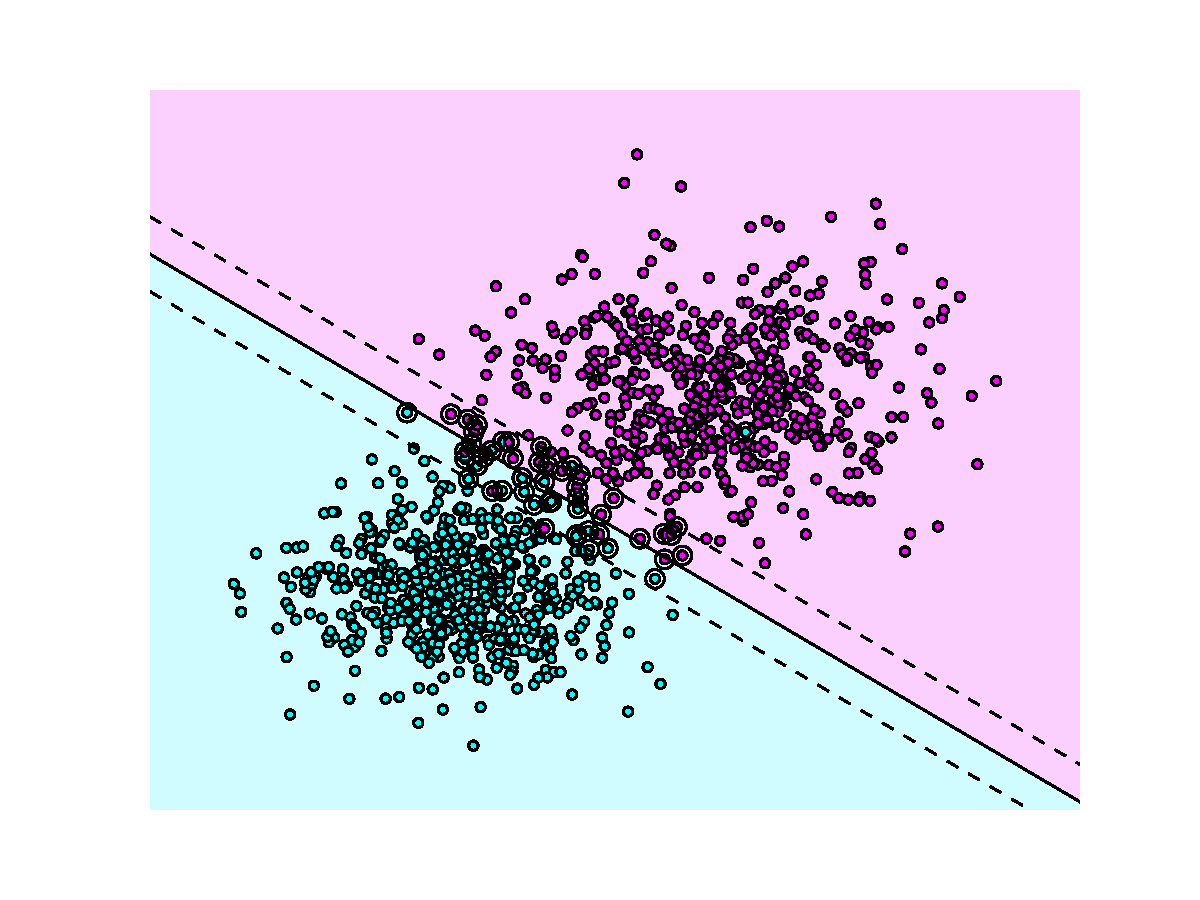
\includegraphics[width=\textwidth]{images/two_class_svm.pdf}
\end{frame}


\begin{frame}
    \frametitle{From Single/Two Class to Multi Class}
    \begin{itemize}
          \item Introduce one SVM classifier ($\textbf{w}_y, b_y$) for each class $y$
          \item For prediction, the maximum scoring classifier determines the label
        \begin{itemize}
              \item[] $\displaystyle y_{\text{predict}} = \argmax_y \;
            \bigl(\left(\textbf{w}_y\right)^{\intercal}\textbf{x} + b_y\bigr) $
        \end{itemize}
    \end{itemize}
\end{frame}


\begin{frame}
    \frametitle{Support Vector Machines - Three Class Example}
    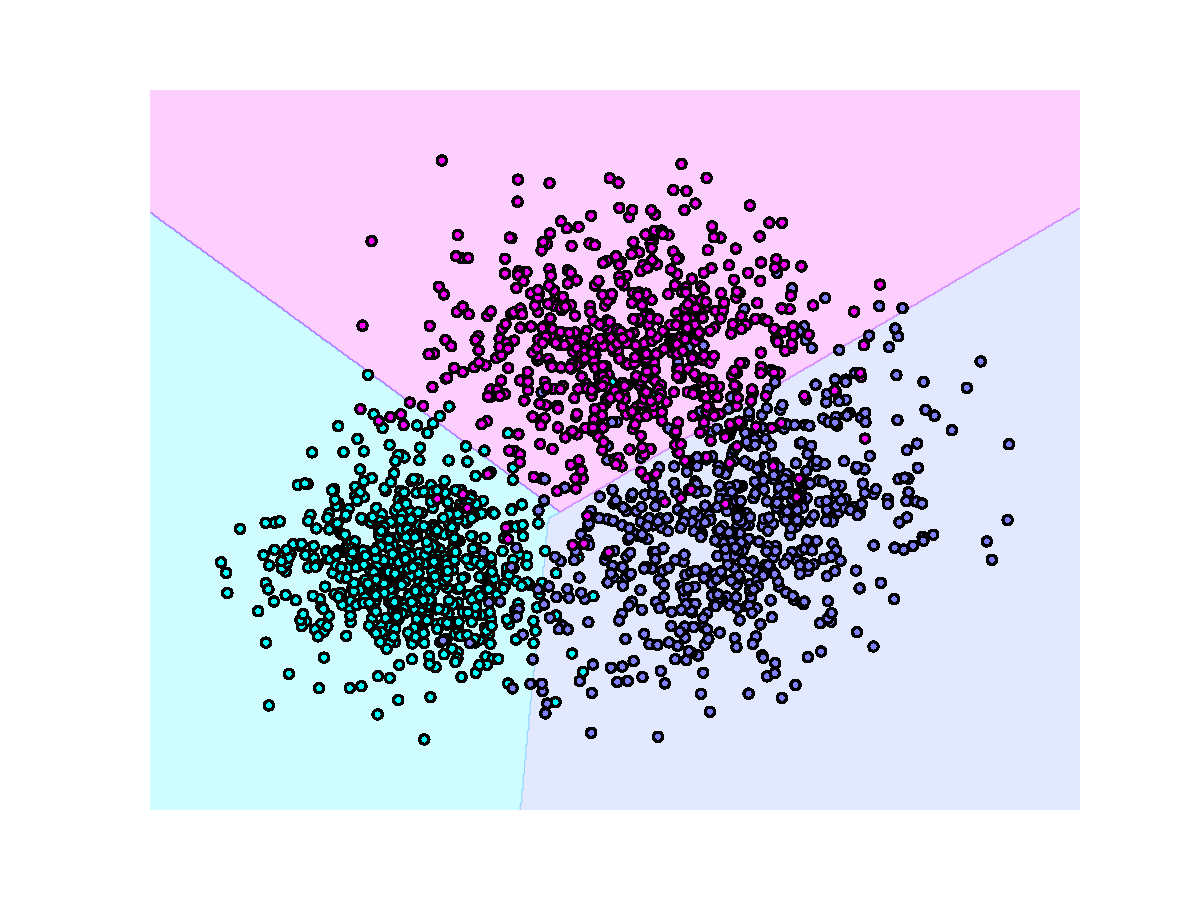
\includegraphics[width=\textwidth]{images/three_class_svm.pdf}
\end{frame}

\begin{frame}
    \frametitle{From SVM to Structured Learning}
    \footfullcite{joachims_04_support}
\end{frame}


%%% Local Variables: 
%%% mode: latex
%%% TeX-master: "../main"
%%% End: 


\section{Use Case - Cell Tracking}

\begin{frame}{Use Case - Cell Tracking}%Cell Tracking - Recap}
    \begin{figure}
        \centering
        \begin{tikzpicture}
            \begin{scope}[baseline=(image1.south)]
                \node[label=above:$t$] (image1) {
                    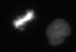
\includegraphics[width=0.25\textwidth]{images/cell_tracking/example_00.png}
                };
                \uncover<2->{
                    \node[transparent_node, red, xshift=-12pt, yshift=5pt] (d11) at (image1.center) {}; 
                    \node[transparent_node, green, xshift=20pt, yshift=-5pt] (d12) at (image1.center) {}; 
                }
            \end{scope}
            \begin{scope}[baseline=(image2.south)]
                \node[right=of image1, xshift=-20pt, label=above:$t+1$] (image2) {
                    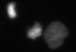
\includegraphics[width=0.25\textwidth]{images/cell_tracking/example_01.png}
                };
                \uncover<3->{
                    \node[transparent_node, red, xshift=-25pt, yshift=15pt] (d21) at (image2.center) {}; 
                    \node[transparent_node, red, xshift=0pt, yshift=-5pt] (d22) at (image2.center) {};
                    \node[transparent_node, green, xshift=18pt, yshift=-10pt] (d23) at (image2.center) {};
                    \path[assignment_arrow, red, bend left=20] (d11) edge (d21);
                    \path[assignment_arrow, red, bend left=10] (d11) edge (d22);
                    \path[assignment_arrow, green, bend right=20] (d12) edge (d23.south west);
                }
            \end{scope}
            \begin{scope}[baseline=(image3.south)]
                \node[right=of image2, xshift=-20pt, label=above:$t+2$] (image3) {
                    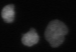
\includegraphics[width=0.25\textwidth]{images/cell_tracking/example_02.png}
                };
                \uncover<4->{
                    \node[transparent_node, red, xshift=-26pt, yshift=13pt] (d31) at (image3.center) {}; 
                    \node[transparent_node, red, xshift=-7pt, yshift=-13pt] (d32) at (image3.center) {};
                    \node[transparent_node, green, xshift=18pt, yshift=-8pt] (d33) at (image3.center) {}; 
                    \path[assignment_arrow, red, bend left=20] (d21) edge (d31);
                    \path[assignment_arrow, red, bend left=20] (d22.north east) edge (d32);
                    \path[assignment_arrow, green, bend right=35] (d23.south east) edge (d33.south west);
                }
            \end{scope}
        \end{tikzpicture}
    \end{figure}
\end{frame}


\begin{frame}
    \frametitle{Tracking Objective Function}
    \begin{center}
        \newcommand{\xShift}{100}
        \newcommand{\yShift}{-30}
        \newcommand{\unaryShift}{-17}
        \begin{tikzpicture}[scale=0.5, every node/.append style={transform shape}]

            \node[detection] (d11) {$X_{1}^{1}$};
            \node[detection, below=of d11, yshift=\yShift] (d12) {$X_{2}^{1}$};

            \node[overlay, unaryfac, above=of d11, yshift=\unaryShift, label=left:$\psi_{\text{det}}(X_1^1)$] (u11) {};
            \node[unaryfac, above=of d12, yshift=\unaryShift] (u12) {};

            \path[unaryfac] (d11) -- (u11);
            \path[unaryfac] (d12) -- (u12);


            \foreach \t in {2,...,3}
            {
                \pgfmathtruncatemacro{\currShift}{(\t * 100)}; 
                \pgfmathtruncatemacro{\prevIndex}{(\t - 1)};
                \node[detection, right=of d\prevIndex1, xshift=\xShift] (d\t1) {$X_{1}^{\t}$};
                \node[detection, below=of d\t1, yshift=\yShift] (d\t2) {$X_{2}^{\t}$};
                \node[detection, below=of d\t2, yshift=\yShift] (d\t3) {$X_{3}^{\t}$};

                \node[unaryfac, above=of d\t1, yshift=\unaryShift] (u\t1) {};
                \node[unaryfac, above=of d\t2, yshift=\unaryShift] (u\t2) {};
                \node[unaryfac, above=of d\t3, yshift=\unaryShift] (u\t3) {};

                \path[unaryfac] (d\t1) -- (u\t1);
                \path[unaryfac] (d\t2) -- (u\t2);
                \path[unaryfac] (d\t3) -- (u\t3);
            }

            \foreach \n in {1,...,2}
            {

                \path[transfac] (d1\n) -- (d2\n);
                \path[transfac] (d2\n) -- (d3\n);

                \node[assignment] (y1\n\n) at ($(d2\n)!0.5!(d1\n)$) {$Z_{\n,\n}^{1}$};
                \node[assignment] (y2\n\n) at ($(d2\n)!0.5!(d3\n)$) {$Z_{\n,\n}^{2}$};

                \node[transfac] (out1\n) at ($(d1\n)!0.5!(y1\n\n)$) {};
                \node[transfac] (out2\n) at ($(d2\n)!0.5!(y2\n\n)$) {};
                \node[transfac] (in2\n) at ($(d2\n)!0.5!(y1\n\n)$) {};
                \node[transfac] (in3\n) at ($(d3\n)!0.5!(y2\n\n)$) {};

                
            }

            \node[transfac, label={[yshift=-10]below:$\psi_{\text{in}}(X_3^2, Z_{\bullet,3}^1)$}] (in23) at (in22|-d23) {};
            \node[transfac] (in33) at (in32|-d33) {};
            \node[transfac, label={[yshift=-10]below:$\psi_{\text{out}}(X_3^2, Z_{3,\bullet}^2)$}] (out23) at (out22|-d23) {};

            \path[transfac] (d23) -- (in23);
            \path[transfac] (d23) -- (out23);
            \path[transfac] (d33) -- (in33);

            \path[transfac] (out23) -- (in33);
            \path[transfac] (out12) -- (in21);
            \path[transfac] (out12) -- (in23);
            \path[transfac] (out23) -- (in32);
            \path[transfac] (out22) -- (in31);
            
            \node[assignment] (y233) at ($(d23)!0.5!(d33)$) {$Z_{3,3}^2$};
            \node[assignment] (y121) at ($(d12)!0.5!(d21)$) {$Z_{2,1}^1$};
            \node[assignment] (y123) at ($(d12)!0.5!(d23)$) {$Z_{2,3}^1$};
            \node[assignment] (y232) at ($(d23)!0.5!(d32)$) {$Z_{3,2}^2$};
            \node[assignment] (y221) at ($(d22)!0.5!(d31)$) {$Z_{2,1}^2$};



        \end{tikzpicture}
    \end{center}
    \begin{align}
        \psi_{k} &= \exp(-E_{k}) \\ \nonumber
        E_{k} &= \dualvec{w}_{k}\VEC{\text{features}}_k \\ \nonumber
        F(\text{data}, Y; \VEC{w}) &= - \sum_k E_k = -\sum_k {\dualvec{w}_Y}_k\VEC{\text{features}}_k
    \end{align}

\end{frame}

\begin{frame}
    \frametitle{Real Tracking Score}
    \newcommand{\trackingExampleScale}{0.35}
    \begin{center}
        \begin{tikzpicture}
            \node (score) { 
\includegraphics[width=0.85\textwidth]{images/struct_svm_objective_4by3_no-cb.pdf} };
            \begin{scope}[x={($(score.south east)-(score.south west)$)},y={($(score.north
                    west)-(score.south west)$)}, overlay]
                \begin{scope}[axis/.style={very thick, ->, >=stealth'}]
                    \draw[axis] (-0.55, -0.5) -- (0.52, -0.5) node (xaxis) [below] {$w_1$};
                    \draw[axis] (-0.5, -0.55) -- (-0.5, 0.52) node (yaxis) [left]  {$w_2$};
                \end{scope}
                \uncover<1->{ \node[score_tracking] (t0) at ( 0.3, -0.15 ) {\begin{tikzpicture}[scale=\trackingExampleScale, every node/.style={transform shape}]
    \begin{scope}[baseline=(image1.south)]
        \node (image1) {
            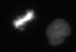
\includegraphics[width=0.25\textwidth]{images/cell_tracking/example_00.png}
        };
        \node[transparent_node, red, xshift=-12pt, yshift=5pt] (d11) at (image1.center) {}; 
        \node[transparent_node, green, xshift=20pt, yshift=-5pt] (d12) at (image1.center) {}; 
    \end{scope}
    \begin{scope}[baseline=(image2.south)]
        \node[right=of image1, xshift=-20pt] (image2) {
            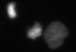
\includegraphics[width=0.25\textwidth]{images/cell_tracking/example_01.png}
        };
        \begin{scope}[overlay]
            \node[transparent_node, red, xshift=-25pt, yshift=15pt] (d21) at (image2.center) {}; 
            \node[transparent_node, red, xshift=0pt, yshift=-5pt] (d22) at (image2.center) {};
            \node[transparent_node, green, xshift=18pt, yshift=-10pt] (d23) at (image2.center) {};
            \path[assignment_arrow, red, bend left=20] (d11) edge (d21);
            \path[assignment_arrow, red, bend left=10] (d11) edge (d22);
            \path[assignment_arrow, green, bend right=20] (d12) edge (d23.south west);
        \end{scope}
    \end{scope}
    \begin{scope}[baseline=(image3.south)]
        \node[right=of image2, xshift=-20pt] (image3) {
            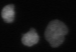
\includegraphics[width=0.25\textwidth]{images/cell_tracking/example_02.png}
        };
        \begin{scope}[overlay]
            \node[transparent_node, red, xshift=-26pt, yshift=13pt] (d31) at (image3.center) {}; 
            \node[transparent_node, red, xshift=-7pt, yshift=-13pt] (d32) at (image3.center) {};
            \node[transparent_node, green, xshift=18pt, yshift=-8pt] (d33) at (image3.center) {}; 
            \path[assignment_arrow, red, bend left=20] (d21) edge (d31);
            \path[assignment_arrow, red, bend left=20] (d22.north east) edge (d32);
            \path[assignment_arrow, green, bend right=35] (d23.south east) edge (d33.south west);
        \end{scope}
    \end{scope}
\end{tikzpicture}


%%% Local Variables: 
%%% mode: latex
%%% TeX-master: "../../../main"
%%% End: 
}; }
                \uncover<2->{ \node[score_tracking] (t1) at ( 0.25, 0.05 ) {\begin{tikzpicture}[scale=\trackingExampleScale, every node/.style={transform shape}]
    \begin{scope}[baseline=(image1.south)]
        \node (image1) {
            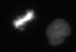
\includegraphics[width=0.25\textwidth]{images/cell_tracking/example_00.png}
        };
        \begin{scope}[overlay]
        \node[transparent_node, red, xshift=-12pt, yshift=5pt] (d11) at (image1.center) {}; 
        \node[transparent_node, green, xshift=20pt, yshift=-5pt] (d12) at (image1.center) {};
        \end{scope}
    \end{scope}
    \begin{scope}[baseline=(image2.south)]
        \node[right=of image1, xshift=-20pt] (image2) {
            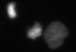
\includegraphics[width=0.25\textwidth]{images/cell_tracking/example_01.png}
        };
        \begin{scope}[overlay]
        \node[transparent_node, red, xshift=-25pt, yshift=15pt] (d21) at (image2.center) {}; 
        \node[transparent_node, red, xshift=0pt, yshift=-5pt] (d22) at (image2.center) {};
        \node[transparent_node, green, xshift=18pt, yshift=-10pt] (d23) at (image2.center) {};
        \path[assignment_arrow, red, bend left=20] (d11) edge (d21);
        \path[assignment_arrow, red, bend left=10] (d11) edge (d22);
        \path[assignment_arrow, green, bend right=20] (d12) edge (d23.south west);
        \end{scope}
    \end{scope}
    \begin{scope}[baseline=(image3.south)]
        \node[right=of image2, xshift=-20pt] (image3) {
            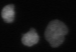
\includegraphics[width=0.25\textwidth]{images/cell_tracking/example_02.png}
        };
        \begin{scope}[overlay]
        \node[transparent_node, red, xshift=-26pt, yshift=13pt] (d31) at (image3.center) {}; 
        \node[transparent_node, red, xshift=-7pt, yshift=-13pt] (d32) at (image3.center) {};
        \path[assignment_arrow, red, bend left=20] (d21) edge (d31);
        \path[assignment_arrow, red, bend left=20] (d22.north east) edge (d32);
        \end{scope}
    \end{scope}
\end{tikzpicture}


%%% Local Variables: 
%%% mode: latex
%%% TeX-master: "../../../main"
%%% End: 
}; }
                \uncover<3->{ \node[score_tracking] (t2) at ( 0.2, 0.4 )  {\begin{tikzpicture}[scale=\trackingExampleScale, every node/.style={transform shape}]
    \begin{scope}[baseline=(image1.south)]
        \node (image1) {
            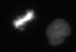
\includegraphics[width=0.25\textwidth]{images/cell_tracking/example_00.png}
        };
    \end{scope}
    \begin{scope}[baseline=(image2.south)]
        \node[right=of image1, xshift=-20pt] (image2) {
            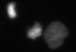
\includegraphics[width=0.25\textwidth]{images/cell_tracking/example_01.png}
        };
    \end{scope}
    \begin{scope}[baseline=(image3.south)]
        \node[right=of image2, xshift=-20pt] (image3) {
            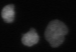
\includegraphics[width=0.25\textwidth]{images/cell_tracking/example_02.png}
        };
    \end{scope}
\end{tikzpicture}


%%% Local Variables: 
%%% mode: latex
%%% TeX-master: "../../../main"
%%% End: 
}; }
                \uncover<4->{ \node[score_tracking] (t3) at ( -0.17, 0.25 ) {\begin{tikzpicture}[scale=\trackingExampleScale, every node/.style={transform shape}]
    \begin{scope}[baseline=(image1.south)]
        \node (image1) {
            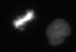
\includegraphics[width=0.25\textwidth]{images/cell_tracking/example_00.png}
        };
        \node[transparent_node, red, xshift=-12pt, yshift=5pt] (d11) at (image1.center) {}; 
        \node[transparent_node, green, xshift=20pt, yshift=-5pt] (d12) at (image1.center) {}; 
    \end{scope}
    \begin{scope}[baseline=(image2.south)]
        \node[right=of image1, xshift=-20pt] (image2) {
            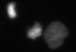
\includegraphics[width=0.25\textwidth]{images/cell_tracking/example_01.png}
        };
        \begin{scope}[overlay]
            \node[transparent_node, red, xshift=-25pt, yshift=15pt] (d21) at (image2.center) {}; 
            \node[transparent_node, green, xshift=0pt, yshift=-5pt] (d22) at (image2.center) {};
            \node[transparent_node, green, xshift=18pt, yshift=-10pt] (d23) at (image2.center) {};
            \path[assignment_arrow, red, bend left=20] (d11) edge (d21);
            \path[assignment_arrow, green, bend left=10] (d12) edge (d22);
            \path[assignment_arrow, green, bend right=20] (d12) edge (d23.south west);
        \end{scope}
    \end{scope}
    \begin{scope}[baseline=(image3.south)]
        \node[right=of image2, xshift=-20pt] (image3) {
            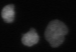
\includegraphics[width=0.25\textwidth]{images/cell_tracking/example_02.png}
        };
        \begin{scope}[overlay]
            \node[transparent_node, red, xshift=-26pt, yshift=13pt] (d31) at (image3.center) {}; 
            \node[transparent_node, green, xshift=-7pt, yshift=-13pt] (d32) at (image3.center) {};
            \node[transparent_node, green, xshift=18pt, yshift=-8pt] (d33) at (image3.center) {}; 
            \path[assignment_arrow, red, bend left=20] (d21) edge (d31);
            \path[assignment_arrow, green, bend left=20] (d22.north east) edge (d32);
            \path[assignment_arrow, green, bend right=35] (d23.south east) edge (d33.south west);
        \end{scope}
    \end{scope}
\end{tikzpicture}


%%% Local Variables: 
%%% mode: latex
%%% TeX-master: "../../../main"
%%% End: 
}; }
                \uncover<5->{ \node[score_tracking] (t4) at ( -0.2, -0.2 ) {\begin{tikzpicture}[scale=\trackingExampleScale, every node/.style={transform shape}]
    \begin{scope}[baseline=(image1.south)]
        \node (image1) {
            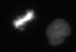
\includegraphics[width=0.25\textwidth]{images/cell_tracking/example_00.png}
        };
        \node[transparent_node, red, xshift=-12pt, yshift=5pt] (d11) at (image1.center) {}; 
        \node[transparent_node, green, xshift=20pt, yshift=-5pt] (d12) at (image1.center) {}; 
    \end{scope}
    \begin{scope}[baseline=(image2.south)]
        \node[right=of image1, xshift=-20pt] (image2) {
            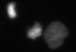
\includegraphics[width=0.25\textwidth]{images/cell_tracking/example_01.png}
        };
        \begin{scope}[overlay]
            \node[transparent_node, red, xshift=-25pt, yshift=15pt] (d21) at (image2.center) {}; 
            \node[transparent_node, green, xshift=18pt, yshift=-10pt] (d23) at (image2.center) {};
            \path[assignment_arrow, red, bend left=20] (d11) edge (d21);
            \path[assignment_arrow, green, bend right=20] (d12) edge (d23.south west);
        \end{scope}
    \end{scope}
    \begin{scope}[baseline=(image3.south)]
        \node[right=of image2, xshift=-20pt] (image3) {
            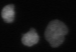
\includegraphics[width=0.25\textwidth]{images/cell_tracking/example_02.png}
        };
        \begin{scope}[overlay]
            \node[transparent_node, red, xshift=-26pt, yshift=13pt] (d31) at (image3.center) {}; 
            \node[transparent_node, green, xshift=18pt, yshift=-8pt] (d33) at (image3.center) {}; 
            \path[assignment_arrow, red, bend left=20] (d21) edge (d31);
            \path[assignment_arrow, green, bend right=35] (d23.south east) edge (d33.south west);
        \end{scope}
    \end{scope}
\end{tikzpicture}


%%% Local Variables: 
%%% mode: latex
%%% TeX-master: "../../../main"
%%% End: 
}; }
                \uncover<6->{
                    \node[font=\small, below=of t0, yshift=31] (w0) {$\textbf{w}^*, b^*$};
                    \node[font=\small, below=of t1, yshift=31] (w1) {$\textbf{w}^{(1)}, b^{(1)}$};
                    \node[font=\small, below=of t2, yshift=31] (w2) {$\textbf{w}^{(2)}, b^{(2)}$};
                    \node[font=\small, below=of t3, yshift=31] (w3) {$\textbf{w}^{(3)}, b^{(3)}$};
                    \node[font=\small, below=of t4, yshift=31] (w4) {$\textbf{w}^{(4)}, b^{(4)}$};
                }
            \end{scope}
        \end{tikzpicture}
    \end{center}

\end{frame}



\begin{frame}
    \frametitle{Tracking Score Obtained From Structured Learning}
    \newcommand{\trackingExampleScale}{0.35}
    \begin{center}
        \begin{tikzpicture}
            \node (score) { 
\includegraphics[width=0.85\textwidth]{images/struct_svm_objective_4by3_no-cb_learned.pdf} };
            \begin{scope}[x={($(score.south east)-(score.south west)$)},y={($(score.north
                    west)-(score.south west)$)}, overlay]
                \begin{scope}[axis/.style={very thick, ->, >=stealth'}]
                    \draw[axis] (-0.55, -0.5) -- (0.52, -0.5) node (xaxis) [below] {$w_1$};
                    \draw[axis] (-0.5, -0.55) -- (-0.5, 0.52) node (yaxis) [left]  {$w_2$};
                \end{scope}
                { \node[score_tracking] (t0) at ( 0.3, -0.15 ) {\begin{tikzpicture}[scale=\trackingExampleScale, every node/.style={transform shape}]
    \begin{scope}[baseline=(image1.south)]
        \node (image1) {
            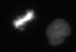
\includegraphics[width=0.25\textwidth]{images/cell_tracking/example_00.png}
        };
        \node[transparent_node, red, xshift=-12pt, yshift=5pt] (d11) at (image1.center) {}; 
        \node[transparent_node, green, xshift=20pt, yshift=-5pt] (d12) at (image1.center) {}; 
    \end{scope}
    \begin{scope}[baseline=(image2.south)]
        \node[right=of image1, xshift=-20pt] (image2) {
            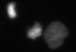
\includegraphics[width=0.25\textwidth]{images/cell_tracking/example_01.png}
        };
        \begin{scope}[overlay]
            \node[transparent_node, red, xshift=-25pt, yshift=15pt] (d21) at (image2.center) {}; 
            \node[transparent_node, red, xshift=0pt, yshift=-5pt] (d22) at (image2.center) {};
            \node[transparent_node, green, xshift=18pt, yshift=-10pt] (d23) at (image2.center) {};
            \path[assignment_arrow, red, bend left=20] (d11) edge (d21);
            \path[assignment_arrow, red, bend left=10] (d11) edge (d22);
            \path[assignment_arrow, green, bend right=20] (d12) edge (d23.south west);
        \end{scope}
    \end{scope}
    \begin{scope}[baseline=(image3.south)]
        \node[right=of image2, xshift=-20pt] (image3) {
            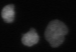
\includegraphics[width=0.25\textwidth]{images/cell_tracking/example_02.png}
        };
        \begin{scope}[overlay]
            \node[transparent_node, red, xshift=-26pt, yshift=13pt] (d31) at (image3.center) {}; 
            \node[transparent_node, red, xshift=-7pt, yshift=-13pt] (d32) at (image3.center) {};
            \node[transparent_node, green, xshift=18pt, yshift=-8pt] (d33) at (image3.center) {}; 
            \path[assignment_arrow, red, bend left=20] (d21) edge (d31);
            \path[assignment_arrow, red, bend left=20] (d22.north east) edge (d32);
            \path[assignment_arrow, green, bend right=35] (d23.south east) edge (d33.south west);
        \end{scope}
    \end{scope}
\end{tikzpicture}


%%% Local Variables: 
%%% mode: latex
%%% TeX-master: "../../../main"
%%% End: 
}; }
                { \node[score_tracking] (t1) at ( 0.25, 0.05 ) {\begin{tikzpicture}[scale=\trackingExampleScale, every node/.style={transform shape}]
    \begin{scope}[baseline=(image1.south)]
        \node (image1) {
            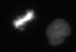
\includegraphics[width=0.25\textwidth]{images/cell_tracking/example_00.png}
        };
        \begin{scope}[overlay]
        \node[transparent_node, red, xshift=-12pt, yshift=5pt] (d11) at (image1.center) {}; 
        \node[transparent_node, green, xshift=20pt, yshift=-5pt] (d12) at (image1.center) {};
        \end{scope}
    \end{scope}
    \begin{scope}[baseline=(image2.south)]
        \node[right=of image1, xshift=-20pt] (image2) {
            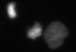
\includegraphics[width=0.25\textwidth]{images/cell_tracking/example_01.png}
        };
        \begin{scope}[overlay]
        \node[transparent_node, red, xshift=-25pt, yshift=15pt] (d21) at (image2.center) {}; 
        \node[transparent_node, red, xshift=0pt, yshift=-5pt] (d22) at (image2.center) {};
        \node[transparent_node, green, xshift=18pt, yshift=-10pt] (d23) at (image2.center) {};
        \path[assignment_arrow, red, bend left=20] (d11) edge (d21);
        \path[assignment_arrow, red, bend left=10] (d11) edge (d22);
        \path[assignment_arrow, green, bend right=20] (d12) edge (d23.south west);
        \end{scope}
    \end{scope}
    \begin{scope}[baseline=(image3.south)]
        \node[right=of image2, xshift=-20pt] (image3) {
            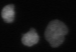
\includegraphics[width=0.25\textwidth]{images/cell_tracking/example_02.png}
        };
        \begin{scope}[overlay]
        \node[transparent_node, red, xshift=-26pt, yshift=13pt] (d31) at (image3.center) {}; 
        \node[transparent_node, red, xshift=-7pt, yshift=-13pt] (d32) at (image3.center) {};
        \path[assignment_arrow, red, bend left=20] (d21) edge (d31);
        \path[assignment_arrow, red, bend left=20] (d22.north east) edge (d32);
        \end{scope}
    \end{scope}
\end{tikzpicture}


%%% Local Variables: 
%%% mode: latex
%%% TeX-master: "../../../main"
%%% End: 
}; }
                { \node[score_tracking] (t2) at ( 0.2, 0.4 )  {\begin{tikzpicture}[scale=\trackingExampleScale, every node/.style={transform shape}]
    \begin{scope}[baseline=(image1.south)]
        \node (image1) {
            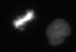
\includegraphics[width=0.25\textwidth]{images/cell_tracking/example_00.png}
        };
    \end{scope}
    \begin{scope}[baseline=(image2.south)]
        \node[right=of image1, xshift=-20pt] (image2) {
            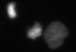
\includegraphics[width=0.25\textwidth]{images/cell_tracking/example_01.png}
        };
    \end{scope}
    \begin{scope}[baseline=(image3.south)]
        \node[right=of image2, xshift=-20pt] (image3) {
            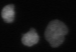
\includegraphics[width=0.25\textwidth]{images/cell_tracking/example_02.png}
        };
    \end{scope}
\end{tikzpicture}


%%% Local Variables: 
%%% mode: latex
%%% TeX-master: "../../../main"
%%% End: 
}; }
                { \node[score_tracking] (t3) at ( -0.17, 0.25 ) {\begin{tikzpicture}[scale=\trackingExampleScale, every node/.style={transform shape}]
    \begin{scope}[baseline=(image1.south)]
        \node (image1) {
            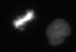
\includegraphics[width=0.25\textwidth]{images/cell_tracking/example_00.png}
        };
        \node[transparent_node, red, xshift=-12pt, yshift=5pt] (d11) at (image1.center) {}; 
        \node[transparent_node, green, xshift=20pt, yshift=-5pt] (d12) at (image1.center) {}; 
    \end{scope}
    \begin{scope}[baseline=(image2.south)]
        \node[right=of image1, xshift=-20pt] (image2) {
            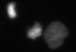
\includegraphics[width=0.25\textwidth]{images/cell_tracking/example_01.png}
        };
        \begin{scope}[overlay]
            \node[transparent_node, red, xshift=-25pt, yshift=15pt] (d21) at (image2.center) {}; 
            \node[transparent_node, green, xshift=0pt, yshift=-5pt] (d22) at (image2.center) {};
            \node[transparent_node, green, xshift=18pt, yshift=-10pt] (d23) at (image2.center) {};
            \path[assignment_arrow, red, bend left=20] (d11) edge (d21);
            \path[assignment_arrow, green, bend left=10] (d12) edge (d22);
            \path[assignment_arrow, green, bend right=20] (d12) edge (d23.south west);
        \end{scope}
    \end{scope}
    \begin{scope}[baseline=(image3.south)]
        \node[right=of image2, xshift=-20pt] (image3) {
            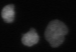
\includegraphics[width=0.25\textwidth]{images/cell_tracking/example_02.png}
        };
        \begin{scope}[overlay]
            \node[transparent_node, red, xshift=-26pt, yshift=13pt] (d31) at (image3.center) {}; 
            \node[transparent_node, green, xshift=-7pt, yshift=-13pt] (d32) at (image3.center) {};
            \node[transparent_node, green, xshift=18pt, yshift=-8pt] (d33) at (image3.center) {}; 
            \path[assignment_arrow, red, bend left=20] (d21) edge (d31);
            \path[assignment_arrow, green, bend left=20] (d22.north east) edge (d32);
            \path[assignment_arrow, green, bend right=35] (d23.south east) edge (d33.south west);
        \end{scope}
    \end{scope}
\end{tikzpicture}


%%% Local Variables: 
%%% mode: latex
%%% TeX-master: "../../../main"
%%% End: 
}; }
                { \node[score_tracking] (t4) at ( -0.2, -0.2 ) {\begin{tikzpicture}[scale=\trackingExampleScale, every node/.style={transform shape}]
    \begin{scope}[baseline=(image1.south)]
        \node (image1) {
            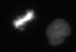
\includegraphics[width=0.25\textwidth]{images/cell_tracking/example_00.png}
        };
        \node[transparent_node, red, xshift=-12pt, yshift=5pt] (d11) at (image1.center) {}; 
        \node[transparent_node, green, xshift=20pt, yshift=-5pt] (d12) at (image1.center) {}; 
    \end{scope}
    \begin{scope}[baseline=(image2.south)]
        \node[right=of image1, xshift=-20pt] (image2) {
            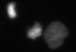
\includegraphics[width=0.25\textwidth]{images/cell_tracking/example_01.png}
        };
        \begin{scope}[overlay]
            \node[transparent_node, red, xshift=-25pt, yshift=15pt] (d21) at (image2.center) {}; 
            \node[transparent_node, green, xshift=18pt, yshift=-10pt] (d23) at (image2.center) {};
            \path[assignment_arrow, red, bend left=20] (d11) edge (d21);
            \path[assignment_arrow, green, bend right=20] (d12) edge (d23.south west);
        \end{scope}
    \end{scope}
    \begin{scope}[baseline=(image3.south)]
        \node[right=of image2, xshift=-20pt] (image3) {
            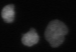
\includegraphics[width=0.25\textwidth]{images/cell_tracking/example_02.png}
        };
        \begin{scope}[overlay]
            \node[transparent_node, red, xshift=-26pt, yshift=13pt] (d31) at (image3.center) {}; 
            \node[transparent_node, green, xshift=18pt, yshift=-8pt] (d33) at (image3.center) {}; 
            \path[assignment_arrow, red, bend left=20] (d21) edge (d31);
            \path[assignment_arrow, green, bend right=35] (d23.south east) edge (d33.south west);
        \end{scope}
    \end{scope}
\end{tikzpicture}


%%% Local Variables: 
%%% mode: latex
%%% TeX-master: "../../../main"
%%% End: 
}; }
                {
                    \node[font=\small, below=of t0, yshift=31] (w0) {$\textbf{w}^*, b^*$};
                    \node[font=\small, below=of t1, yshift=31] (w1) {$\textbf{w}^{(1)}, b^{(1)}$};
                    \node[font=\small, below=of t2, yshift=31] (w2) {$\textbf{w}^{(2)}, b^{(2)}$};
                    \node[font=\small, below=of t3, yshift=31] (w3) {$\textbf{w}^{(3)}, b^{(3)}$};
                    \node[font=\small, below=of t4, yshift=31] (w4) {$\textbf{w}^{(4)}, b^{(4)}$};
                }
            \end{scope}
        \end{tikzpicture}
    \end{center}

\end{frame}



\begin{frame}
    \frametitle{Struct SVM Tracking Score Function Augmented By Hamming Loss}

    \begin{itemize}
          \item Incorporate hamming loss in original objective to solve $\displaystyle
        \max_{Y\in Y_i}\bigl(\Delta(Y, Y_i) + F( \VEC{x}_i, Y) \bigr)$
    \end{itemize}

    \begin{center}
        \newcommand{\xShift}{100}
        \newcommand{\yShift}{-30}
        \newcommand{\unaryXShift}{22}
        \newcommand{\unaryShift}{-\unaryXShift}
        \begin{tikzpicture}[scale=0.5, every node/.append style={transform shape}]

            \node[detection] (d11) {$X_{1}^{1}$};
            \node[detection, below=of d11, yshift=\yShift] (d12) {$X_{2}^{1}$};

            \node[overlay, unaryfac, above left=of d11, yshift=\unaryShift, xshift=\unaryXShift, label=left:$\psi_{\text{det}}(X_1^1)$] (u11) {};
            \node[unaryfac, above left=of d12, yshift=\unaryShift, xshift=\unaryXShift] (u12) {};

            \path[unaryfac] (d11) -- (u11);
            \path[unaryfac] (d12) -- (u12);

            \node[lossfac, above right=of d11, yshift=\unaryShift, xshift=-\unaryXShift,
            label=right:$\Delta$] (l11) {}; 
            \node[lossfac, above right=of d12, yshift=\unaryShift, xshift=-\unaryXShift] (l12) {};

            \path[lossfac] (d11) -- (l11);
            \path[lossfac] (d12) -- (l12);


            \foreach \t in {2,...,3}
            {
                \pgfmathtruncatemacro{\currShift}{(\t * 100)}; 
                \pgfmathtruncatemacro{\prevIndex}{(\t - 1)};
                \node[detection, right=of d\prevIndex1, xshift=\xShift] (d\t1) {$X_{1}^{\t}$};
                \node[detection, below=of d\t1, yshift=\yShift] (d\t2) {$X_{2}^{\t}$};
                \node[detection, below=of d\t2, yshift=\yShift] (d\t3) {$X_{3}^{\t}$};

                \node[unaryfac, above left=of d\t1, yshift=\unaryShift, xshift=\unaryXShift] (u\t1) {};
                \node[unaryfac, above left=of d\t2, yshift=\unaryShift, xshift=\unaryXShift] (u\t2) {};
                \node[unaryfac, above left=of d\t3, yshift=\unaryShift, xshift=\unaryXShift] (u\t3) {};

                \node[lossfac, above right=of d\t1, yshift=\unaryShift, xshift=-\unaryXShift] (l\t1) {};
                \node[lossfac, above right=of d\t2, yshift=\unaryShift, xshift=-\unaryXShift] (l\t2) {};
                \node[lossfac, above right=of d\t3, yshift=\unaryShift, xshift=-\unaryXShift] (l\t3) {};

                \path[unaryfac] (d\t1) -- (u\t1);
                \path[unaryfac] (d\t2) -- (u\t2);
                \path[unaryfac] (d\t3) -- (u\t3);

                \path[lossfac] (d\t1) -- (l\t1);
                \path[lossfac] (d\t2) -- (l\t2);
                \path[lossfac] (d\t3) -- (l\t3);
            }

            \foreach \n in {1,...,2}
            {

                \path[transfac] (d1\n) -- (d2\n);
                \path[transfac] (d2\n) -- (d3\n);

                \node[assignment] (y1\n\n) at ($(d2\n)!0.5!(d1\n)$) {$Z_{\n,\n}^{1}$};
                \node[assignment] (y2\n\n) at ($(d2\n)!0.5!(d3\n)$) {$Z_{\n,\n}^{2}$};

                \node[transfac] (out1\n) at ($(d1\n)!0.5!(y1\n\n)$) {};
                \node[transfac] (out2\n) at ($(d2\n)!0.5!(y2\n\n)$) {};
                \node[transfac] (in2\n) at ($(d2\n)!0.5!(y1\n\n)$) {};
                \node[transfac] (in3\n) at ($(d3\n)!0.5!(y2\n\n)$) {};

                \node[lossfac, above right=of y1\n\n, yshift=\unaryShift, xshift=-\unaryXShift]
                (l1\n\n) {};
                \node[lossfac, above right=of y2\n\n, yshift=\unaryShift, xshift=-\unaryXShift]
                (l2\n\n) {};

                \path[lossfac] (y1\n\n) -- (l1\n\n);
                \path[lossfac] (y2\n\n) -- (l2\n\n);
                
            }

            \node[transfac, label={[yshift=-10]below:$\psi_{\text{in}}(X_3^2, Z_{\bullet,3}^1)$}] (in23) at (in22|-d23) {};
            \node[transfac] (in33) at (in32|-d33) {};
            \node[transfac, label={[yshift=-10]below:$\psi_{\text{out}}(X_3^2, Z_{3,\bullet}^2)$}] (out23) at (out22|-d23) {};

            \path[transfac] (d23) -- (in23);
            \path[transfac] (d23) -- (out23);
            \path[transfac] (d33) -- (in33);

            \path[transfac] (out23) -- (in33);
            \path[transfac] (out12) -- (in21);
            \path[transfac] (out12) -- (in23);
            \path[transfac] (out23) -- (in32);
            \path[transfac] (out22) -- (in31);
            
            \node[assignment] (y233) at ($(d23)!0.5!(d33)$) {$Z_{3,3}^2$};
            \node[assignment] (y121) at ($(d12)!0.5!(d21)$) {$Z_{2,1}^1$};
            \node[assignment] (y123) at ($(d12)!0.5!(d23)$) {$Z_{2,3}^1$};
            \node[assignment] (y232) at ($(d23)!0.5!(d32)$) {$Z_{3,2}^2$};
            \node[assignment] (y221) at ($(d22)!0.5!(d31)$) {$Z_{2,1}^2$};

            \node[lossfac, above right=of y233, yshift=\unaryShift, xshift=-\unaryXShift]
            (l233) {};
            \node[lossfac, above left=of y121, yshift=\unaryShift, xshift=\unaryXShift]
            (l121) {};
            \node[lossfac, above right=of y123, yshift=\unaryShift, xshift=-\unaryXShift]
            (l123) {};
            \node[lossfac, above left=of y232, yshift=\unaryShift, xshift=\unaryXShift]
            (l232) {};
            \node[lossfac, above left=of y221, yshift=\unaryShift, xshift=\unaryXShift]
            (l221) {};

            \path[lossfac] (y233) -- (l233);
            \path[lossfac] (y121) -- (l121);
            \path[lossfac] (y123) -- (l123);
            \path[lossfac] (y232) -- (l232);
            \path[lossfac] (y221) -- (l221);

        \end{tikzpicture}
    \end{center}

\end{frame}



\begin{frame}
    \frametitle{Struct SVM Tracking Score Function Augmented By Higher Order Loss}

    \begin{itemize}
          \item Incorporate higher order loss in original objective to solve $\displaystyle
        \max_{Y\in Y_i}\bigl(\Delta(Y, Y_i) + F( \VEC{x}_i, Y) \bigr)$
    \end{itemize}

    \begin{center}
        \newcommand{\xShift}{100}
        \newcommand{\yShift}{-30}
        \newcommand{\unaryXShift}{22}
        \newcommand{\unaryShift}{-\unaryXShift}
        \begin{tikzpicture}[scale=0.5, every node/.append style={transform shape}]

            \node[detection] (d11) {$X_{1}^{1}$};
            \node[detection, below=of d11, yshift=\yShift] (d12) {$X_{2}^{1}$};

            \node[overlay, unaryfac, above left=of d11, yshift=\unaryShift, xshift=\unaryXShift, label=left:$\psi_{\text{det}}(X_1^1)$] (u11) {};
            \node[unaryfac, above left=of d12, yshift=\unaryShift, xshift=\unaryXShift] (u12) {};

            \path[unaryfac] (d11) -- (u11);
            \path[unaryfac] (d12) -- (u12);

            \foreach \t in {2,...,3}
            {
                \pgfmathtruncatemacro{\currShift}{(\t * 100)}; 
                \pgfmathtruncatemacro{\prevIndex}{(\t - 1)};
                \node[detection, right=of d\prevIndex1, xshift=\xShift] (d\t1) {$X_{1}^{\t}$};
                \node[detection, below=of d\t1, yshift=\yShift] (d\t2) {$X_{2}^{\t}$};
                \node[detection, below=of d\t2, yshift=\yShift] (d\t3) {$X_{3}^{\t}$};

                \node[unaryfac, above left=of d\t1, yshift=\unaryShift, xshift=\unaryXShift] (u\t1) {};
                \node[unaryfac, above left=of d\t2, yshift=\unaryShift, xshift=\unaryXShift] (u\t2) {};
                \node[unaryfac, above left=of d\t3, yshift=\unaryShift, xshift=\unaryXShift] (u\t3) {};

                \path[unaryfac] (d\t1) -- (u\t1);
                \path[unaryfac] (d\t2) -- (u\t2);
                \path[unaryfac] (d\t3) -- (u\t3);

            }

            \foreach \n in {1,...,2}
            {

                \path[transfac] (d1\n) -- (d2\n);
                \path[transfac] (d2\n) -- (d3\n);

                \node[assignment] (y1\n\n) at ($(d2\n)!0.5!(d1\n)$) {$Z_{\n,\n}^{1}$};
                \node[assignment] (y2\n\n) at ($(d2\n)!0.5!(d3\n)$) {$Z_{\n,\n}^{2}$};

                \node[transfac] (out1\n) at ($(d1\n)!0.5!(y1\n\n)$) {};
                \node[transfac] (out2\n) at ($(d2\n)!0.5!(y2\n\n)$) {};
                \node[transfac] (in2\n) at ($(d2\n)!0.5!(y1\n\n)$) {};
                \node[transfac] (in3\n) at ($(d3\n)!0.5!(y2\n\n)$) {};

            }

            \node[transfac, label={[yshift=-10]below:$\psi_{\text{in}}(X_3^2, Z_{\bullet,3}^1)$}] (in23) at (in22|-d23) {};
            \node[transfac] (in33) at (in32|-d33) {};
            \node[transfac, label={[yshift=-10]below:$\psi_{\text{out}}(X_3^2, Z_{3,\bullet}^2)$}] (out23) at (out22|-d23) {};

            \path[transfac] (d23) -- (in23);
            \path[transfac] (d23) -- (out23);
            \path[transfac] (d33) -- (in33);

            \path[transfac] (out23) -- (in33);
            \path[transfac] (out12) -- (in21);
            \path[transfac] (out12) -- (in23);
            \path[transfac] (out23) -- (in32);
            \path[transfac] (out22) -- (in31);
            
            \node[assignment] (y233) at ($(d23)!0.5!(d33)$) {$Z_{3,3}^2$};
            \node[assignment] (y121) at ($(d12)!0.5!(d21)$) {$Z_{2,1}^1$};
            \node[assignment] (y123) at ($(d12)!0.5!(d23)$) {$Z_{2,3}^1$};
            \node[assignment] (y232) at ($(d23)!0.5!(d32)$) {$Z_{3,2}^2$};
            \node[assignment] (y221) at ($(d22)!0.5!(d31)$) {$Z_{2,1}^2$};

            \begin{pgfonlayer}{background}
                \begin{scope}[overlay]
                    \node[lossfac, label=below left:$\Delta$] at (d12|-d23) (l) {};

                    \path[lossfac] (d11) edge[bend right=32] (l);
                    \path[lossfac] (d12) -- (l);
                    \path[lossfac] (d21) edge[bend right=10] (l);
                    \path[lossfac] (d22) edge[bend right=10] (l);
                    \path[lossfac] (d23) edge[bend left=12] (l);
                    \path[lossfac] (d31) edge[bend left=12] (l);
                    \path[lossfac] (d32) edge (l);
                    \path[lossfac] (d33) edge[bend left=25] (l);

                    \path[lossfac] (y111) edge[bend right=5] (l);
                    \path[lossfac] (y121) edge (l);
                    \path[lossfac] (y122) edge (l);
                    \path[lossfac] (y123) edge (l);
                    \path[lossfac] (y211) edge[bend right=5] (l);
                    \path[lossfac] (y221) edge[bend right=15]  (l);
                    \path[lossfac] (y232) edge (l);
                    \path[lossfac] (y233) edge[bend left=17] (l);
                    \path[lossfac] (y222) edge (l);
                    
                \end{scope}
            \end{pgfonlayer}
        \end{tikzpicture}
    \end{center}

\end{frame}

\begin{frame}
    \frametitle{Wrap-Up}
    \begin{itemize}
          \item Structured Prediction
          \item[] $\displaystyle Y_{\text{predict}} = \argmax_Y\ \structSvmScore $
          \item Structured Learning
        \begin{align*}
            &\min_{\VEC{w}, \xi} \frac{1}{2}\dualvec{w}\VEC{w} + \frac{C}{kN} \sum_{i=1}^N(\xi_i)^k
            , \; \; \st \\ \nonumber
            &F(\VEC{x}_i, Y_i) - F(\VEC{x}_i, Y) \ge \Delta(Y, Y_i) - \xi_i \; \; \forall i, \; \forall Y \in \mathcal{Y}\setminus Y_i 
        \end{align*}
        \item Augment original model by loss to keep implementation effort low. Do not forget about
      tractability!
        \item[] $\Delta(Y, Y_i) + F( \VEC{x}_i, Y)$
    \end{itemize}
\end{frame}


\begin{frame}
    \frametitle{Acknowledgments}
    \begin{itemize}
          \item HCI Heidelberg - Tracking
        \begin{itemize}
              \item[] Martin Schiegg
              \item[] Carsten Haubold
        \end{itemize}
          \item ETH Z\"urich - Segmentation
        \begin{itemize}
              \item[] Jan Funke
        \end{itemize}
          \item HCI Heidelberg - OpenGM
        \begin{itemize}
              \item[] J\"org Kappes
              \item[] Thorsten Beier
        \end{itemize}
    \end{itemize}
\end{frame}


    %%% Local Variables: 
    %%% mode: latex
    %%% TeX-master: "../main"
    %%% End: 


\appendix % OPTIONAL
\newcounter{finalframe}
\setcounter{finalframe}{\value{framenumber}}

% \input{content/backup}

\setcounter{framenumber}{\value{finalframe}}

\end{document}



%%% Local Variables: 
%%% mode: latex
%%% TeX-master: t
%%% End: 
